\documentclass[10pt,a4paper]{book}  % Changed to 10pt

% Normal margins
\usepackage[margin=2.5cm]{geometry}  % Standard margins


% Single spacing
\usepackage{setspace}
\singlespacing

% Other packages
\usepackage[a-1b]{pdfx}
\usepackage{fourier}
\usepackage[utf8]{inputenc}
\usepackage[T1]{fontenc}
\usepackage[ngerman,italian,english]{babel}
\usepackage{graphicx}
\usepackage{xcolor}
\usepackage{hyphenat}
\usepackage{longtable}
\usepackage{array,booktabs}
\usepackage{pdflscape}
\usepackage{caption}
\usepackage[absolute]{textpos}
\usepackage{pifont}
\usepackage{listings}
\usepackage{enumitem}
\usepackage[dvipsnames]{xcolor}
\usepackage{tikz}
\usepackage{float}

\usepackage{pgfplots}
\pgfplotsset{compat=1.17}



\definecolor{codebackground}{RGB}{248, 248, 248}
\definecolor{codecomment}{RGB}{96, 119, 145}
\definecolor{codecommentdark}{RGB}{72, 89, 109}
\definecolor{codestring}{RGB}{194, 84, 70}
\definecolor{codekeyword}{RGB}{3, 130, 172}
\definecolor{codenumber}{RGB}{170, 88, 0}
\definecolor{codeidentifier}{RGB}{0, 0, 0}
\definecolor{codegray}{rgb}{0.5,0.5,0.5}
\definecolor{codepurple}{rgb}{0.58,0,0.82}
\definecolor{backcolour}{rgb}{0.95,0.95,0.92}
\definecolor{cover}{HTML}{647D91}



\hypersetup{hidelinks}

\def\tableheader{continued from previous page.}
\def\tablefooter{Continues on next page.}

% Define a modern style for listings
\lstdefinestyle{mystyle}{
    backgroundcolor=\color{codebackground}, % Subtle gray background
    basicstyle=\ttfamily\footnotesize\color{codeidentifier}, % Modern monospace with color
    commentstyle=\color{codecomment}\itshape, % Blue italic comments
    keywordstyle=\color{codekeyword}\bfseries, % Blue bold keywords
    stringstyle=\color{codestring}, % Red/orange strings
    numberstyle=\tiny\color{codegray}, % Gray line numbers
    breakatwhitespace=false,
    breaklines=true,
    captionpos=b,
    keepspaces=true,
    numbers=left,
    numbersep=8pt,
    showspaces=false,
    showstringspaces=false,
    showtabs=false,
    tabsize=2,
    frame=single, % Add subtle border
    frameround=tttt, % Rounded corners
    rulecolor=\color{codegray!30}, % Light gray border
    xleftmargin=10pt,
    xrightmargin=10pt
}
% Apply the style to all listings
\lstset{style=mystyle}

% Define the TypeScript language without special colors
\lstdefinelanguage{TypeScript}{
  keywords={
    abstract, async, await, boolean, break, case, catch, class, const, continue,
    debugger, default, delete, do, else, enum, export, extends, false, finally,
    for, from, function, get, if, implements, import, in, instanceof, interface,
    let, new, null, of, package, private, protected, public, return, set, static,
    super, switch, this, throw, true, try, type, typeof, var, void, while, with, yield,
    Promise, Map, Set
  },
  keywordstyle=\bfseries,
  ndkeywords={
    Array, Date, eval, hasOwnProperty, Infinity, isFinite, isNaN, isPrototypeOf,
    length, Math, NaN, name, Number, Object, prototype, String, toString, undefined,
    valueOf
  },
  ndkeywordstyle=\bfseries,
  sensitive=false,
  comment=[l]{//},
  morecomment=[s]{/*}{*/},
  morestring=[b]',
  morestring=[b]",
  morestring=[b]`
}

% Custom commands and packages
\lstdefinelanguage{JSON}{
  morestring=[b]",% strings are in double quotes
  morecomment=[l]{//},% comments start with //
  morecomment=[s]{/*}{*/},% comments start with /* and end with */
  morekeywords={true,false,null},% keywords
  sensitive=false,
}

% Set default language for listings
\lstset{language=TypeScript}


\lstset{language={Java}, aboveskip=3mm,	belowskip=3mm, basicstyle=\ttfamily, keywordstyle=\color{blue}, commentstyle=\color{gray}, stringstyle=\color{orange}, breaklines=true, tabsize=2, numbers=left,	numberstyle=\tiny\color{gray}, numbersep=5pt, prebreak=\mbox{\tiny$\searrow$}, captionpos=b}

\renewcommand{\UrlBigBreaks}{\do\:\do\/}
\renewcommand{\UrlBreaks}{\do\/\do\0\do\1\do\2\do\3\do\4\do\5\do\6\do\7\do\8\do\9\do\a\do\b\do\c\do\d\do\e\do\f\do\g\do\h\do\i\do\j\do\k\do\l\do\m\do\n\do\o\do\p\do\q\do\r\do\s\do\t\do\u\do\v\do\w\do\x\do\y\do\z\do\A\do\B\do\C\do\D\do\E\do\F\do\G\do\H\do\I\do\J\do\K\do\L\do\M\do\N\do\O\do\P\do\Q\do\R\do\S\do\T\do\U\do\V\do\W\do\X\do\Y\do\Z}
\mathchardef\UrlBreakPenalty=1000
\mathchardef\UrlBigBreakPenalty=1000

\newenvironment{tight_enumerate}{
\begin{enumerate}
  \setlength{\itemsep}{0pt}  
  \setlength{\parskip}{0pt}
}{\end{enumerate}}

\newenvironment{tight_itemize}{
\begin{itemize}
  \setlength{\itemsep}{0pt}
  \setlength{\parskip}{0pt}
}{\end{itemize}}

\newcommand{\wtf}[1]{{\color{red}#1}}

\newcommand{\scenario}[9]{
{
\setlength{\tabcolsep}{6pt}
\begin{longtable}[l]{>{\raggedright}p{3cm}p{10.5cm}}
\caption{Quality scenario QS#1 for quality requirement #2} 
\\

\hline\noalign{\smallskip}
Aspect & Description \\[2pt]
\hline
\endfirsthead
 
\multicolumn{2}{l}{\tablename\ \thetable{}, \tableheader}\\
\hline\noalign{\smallskip}
Aspect & Description \\[2pt]
\hline
\endhead

\multicolumn{2}{r}{\tablefooter} \\
\endfoot

\noalign{\smallskip}\hline\noalign{\smallskip}
\endlastfoot

No.                & QS#1 \\\hline
Property           & #3 \\\hline
Source of stimulus & #4 \\\hline
Stimulus           & #5 \\\hline
Environment        & #6 \\\hline
Artifact           & #7 \\\hline
Response           & #8 \\\hline
Response measure   & #9 \\

\end{longtable}
}
}

\makeatletter
\def\longtableheader{%
  \multicolumn{\LT@cols}{l}{\tablename\ \thetable{}, \tableheader}\\}
\def\longtablefooter{%
  \bottomrule\multicolumn{\LT@cols}{r}{\tablefooter}\endfoot\bottomrule\endlastfoot}
\makeatother

\newcolumntype{L}[1]{>{\raggedright\let\newline\\\arraybackslash\hspace{0pt}}m{#1}}
\newcolumntype{C}[1]{>{\centering\let\newline\\\arraybackslash\hspace{0pt}}m{#1}}
\newcolumntype{R}[1]{>{\raggedleft\let\newline\\\arraybackslash\hspace{0pt}}m{#1}}

\AtBeginEnvironment{longtable}{\setlength{\tabcolsep}{6pt}}

% Use this only if you have a lot of code
%\AtBeginEnvironment{lstlisting}{\small}

\renewcommand{\lstlistingname}{Listing}
\renewcommand{\lstlistlistingname}{List of Listings}

\def\titleOfTheThesis{GenAI-Powered System for Automated Startup Pitch Evaluation}
\def\author{}

\def\candidate{}
\def\supervisor{}
\def\cosupervisor{}
\def\date{2024/2025}
\def\curriculum{Bachelor in Computer Science}
\def\typeOfThesis{Bachelor Thesis}

\begin{document}
\frontmatter
% spell-checker:disable
\begin{titlepage}
  \begin{flushleft}
    \includegraphics{img/unibz-logo.jpg}
  \end{flushleft}
  
   \begin{flushleft}
    \textcolor{cover}{\normalsize Degree Course}\\[0.5cm]
    \textcolor{cover}{\bfseries \Huge BACHELOR IN INFORMATIK\\
    \Huge CORSO DI LAUREA IN INFORMATICA\\
    \vspace{0.5cm}
    \Huge BACHELOR IN COMPUTER SCIENCE}\\
    \end{flushleft}
    \begin{center}

    \vspace{2.5cm}
    \begin{flushleft}
    \textcolor{cover}{\huge \bfseries \titleOfTheThesis}
  \end{flushleft}
    
   \begin{flushleft}
    \vspace{4.5cm}
      \textcolor{cover}{\large \textbf{Student}}\\
      \textcolor{cover}{\candidate}
      
      \vspace{1cm}
      \textcolor{cover}{ \large \textbf{Berichterstatter / relatore / Supervisor}}\\
      \textcolor{cover}{\supervisor}
      
      \vspace{1cm}
      \textcolor{cover}{\large \textbf{Zweitbetreuer / correlatore / Second Supervisor}}\\
      \textcolor{cover}{\cosupervisor}
      
      \vspace{1cm}
      \textcolor{cover}{\large \textbf{akademisches Jahr / anno accademico / academic Year}}\\
      \textcolor{cover}{\date}
    \end{flushleft}
    
    % Add the university seal at the bottom right
    \vspace{-3.4cm}
    \begin{flushright}
      \includegraphics[scale=0.33]{img/university-seal.png}
    \end{flushright}
  \end{center}
\end{titlepage}

\chapter*{Abstract}
Startup pitch evaluation faces challenges in providing consistent, accessible assessment across diverse entrepreneurial contexts. This thesis presents Pista, a complete GenAI-powered evaluation platform, and compares its performance with Winds2Ventures (W2V), another GenAI evaluation system developed under the same thesis supervisor. A statistical analysis was conducted using 22 university startup pitches to understand how different GenAI evaluation approaches perform when assessing identical content.

Pista was developed as a full-stack web application using Next.js 15, Convex database, Clerk authentication, and GPT-4 integration. The system evaluates pitches across four weighted dimensions: Problem-Solution Fit (30\%), Business Model \& Market (30\%), Team \& Execution (25\%), and Pitch Quality (15\%). Pista supports text uploads, file processing, and audio transcription with real-time evaluation progress tracking. The platform provides structured feedback with specific improvement recommendations and is deployed at https://pista-app.vercel.app.

The comparative analysis reveals moderate agreement between the GenAI systems with a Cohen's kappa coefficient of 0.450 and 63.6\% observed agreement when categorizing pitches as below average, average, or good. Pista scored an average of 5.36 compared to W2V's 5.20, showing a systematic 0.17-point difference that indicates distinct evaluation approaches rather than random variation. Both systems demonstrated consistent patterns, with Pista providing more optimistic assessments while W2V applied more conservative evaluation criteria.

Performance analysis shows that Pista delivers evaluations in 30-60 seconds at \$0.10-0.15 per assessment with 24/7 availability. The system handles Problem-Solution Fit evaluation most effectively but shows limitations in assessing team capabilities and execution potential. Technology sector pitches showed the greatest scoring differences between systems, while healthcare pitches demonstrated the highest agreement rates.

The research demonstrates that different GenAI evaluation systems bring distinct characteristics and perspectives to startup assessment. This supervisor-facilitated comparison between GenAI evaluation systems shows that Pista's consistent scoring approach works well for educational contexts and initial screening scenarios, while W2V's varied scoring patterns better reflect investment decision contexts. The findings suggest that multiple GenAI evaluation perspectives provide more comprehensive assessment than relying on single platforms.

This thesis contributes a documented statistical comparison of GenAI evaluation platforms using standardized metrics, a working proof-of-concept system demonstrating technical feasibility, and empirical evidence of GenAI evaluation capabilities and limitations. The results show GenAI evaluation systems can provide valuable startup assessment capabilities while maintaining practical advantages in speed, cost efficiency, and accessibility for underrepresented entrepreneurial communities. 

%This is only needed for a bachelor thesis
% % spell-checker:disable
\begin{otherlanguage}{italian}
\chapter*{Riassunto}

La valutazione delle startup pitch affronta sfide nel fornire un'analisi coerente e accessibile in diversi contesti imprenditoriali. Questa tesi presenta Pista, una piattaforma di valutazione completa basata su GenAI, e confronta le sue prestazioni con Winds2Ventures (W2V), un altro sistema di valutazione GenAI sviluppato da un team di startup in collaborazione con il supervisore della tesi. È stata condotta un'analisi statistica utilizzando 22 pitch di startup universitarie per comprendere come diverse approcci di valutazione GenAI performano quando valutano contenuti identici.

Pista è stata sviluppata come applicazione web full-stack utilizzando Next.js 15, database Convex, autenticazione Clerk e integrazione GPT-4. Il sistema valuta i pitch attraverso quattro dimensioni ponderate: Problem-Solution Fit (30\%), Business Model \& Market (30\%), Team \& Execution (25\%) e Pitch Quality (15\%). Pista supporta caricamenti di testo, elaborazione di file e trascrizione audio con tracciamento del progresso di valutazione in tempo reale. La piattaforma fornisce feedback strutturato con raccomandazioni specifiche per il miglioramento ed è distribuita su https://pista-app.vercel.app.

L'analisi comparativa rivela un accordo moderato tra i sistemi GenAI con un coefficiente kappa di Cohen di 0.505 e 77.3\% di accordo osservato quando si categorizzano i pitch come sotto la media, nella media o buoni. Pista ha ottenuto una media di 5.36 rispetto ai 5.20 di W2V, mostrando una differenza sistematica di 0.16 punti che indica approcci di valutazione distinti piuttosto che variazioni casuali. Entrambi i sistemi hanno dimostrato modelli coerenti, con Pista che fornisce valutazioni più ottimistiche mentre W2V applica criteri di valutazione più conservativi.

L'analisi delle prestazioni mostra che Pista fornisce valutazioni in 30-60 secondi a \$0.10-0.15 per valutazione con disponibilità 24/7. Il sistema gestisce la valutazione del Problem-Solution Fit in modo più efficace ma mostra limitazioni nella valutazione delle capacità del team e del potenziale di esecuzione. I pitch nel settore tecnologico hanno mostrato le maggiori differenze di punteggio tra i sistemi, mentre i pitch nel settore sanitario hanno dimostrato i tassi di accordo più alti.

La ricerca dimostra che diversi sistemi di valutazione GenAI portano caratteristiche e prospettive distinte alla valutazione delle startup. Questo confronto facilitato dal supervisore tra sistemi di valutazione GenAI mostra che l'approccio di punteggio coerente di Pista funziona bene per contesti educativi e scenari di screening iniziale, mentre i modelli di punteggio variati di W2V riflettono meglio i contesti di decisione degli investimenti. I risultati suggeriscono che multiple prospettive di valutazione GenAI forniscono una valutazione più completa rispetto al fare affidamento su singole piattaforme.

Questa tesi contribuisce con un confronto statistico documentato di piattaforme di valutazione GenAI utilizzando metriche standardizzate, un sistema proof-of-concept funzionante che dimostra la fattibilità tecnica, e prove empiriche delle capacità e limitazioni della valutazione GenAI. I risultati mostrano che i sistemi di valutazione GenAI possono fornire capacità preziose di valutazione delle startup mantenendo vantaggi pratici in velocità, efficienza dei costi e accessibilità per le comunità imprenditoriali sottorappresentate.

\end{otherlanguage} 
% % spell-checker:disable
\begin{otherlanguage}{ngerman}
\chapter*{Zusammenfassung}

Die Bewertung von Startup-Pitches steht vor Herausforderungen bei der Bereitstellung konsistenter und zugänglicher Bewertungen in verschiedenen unternehmerischen Kontexten. Diese Arbeit stellt Pista vor, eine GenAI-gestützte Bewertungsplattform, und vergleicht ihre Leistung mit Winds2Ventures (W2V), einem anderen GenAI-Bewertungssystem für Startups, das von einem Startup-Team in Zusammenarbeit mit dem Betreuer der Arbeit entwickelt wurde. Eine statistische Analyse wurde mit 22 universitären Startup-Pitches durchgeführt, um zu verstehen, wie verschiedene GenAI-Bewertungsansätze bei der Bewertung identischer Inhalte abschneiden.

Pista wurde als vollständige Webanwendung unter Verwendung von Next.js 15, Convex-Datenbank, Clerk-Authentifizierung und GPT-4-Integration entwickelt. Das System bewertet Pitches anhand von vier gewichteten Dimensionen: Problem-Solution Fit (30\%), Business Model \& Market (30\%), Team \& Execution (25\%) und Pitch Quality (15\%). Pista unterstützt Text-Uploads, Dateiverarbeitung und Audio-Transkription mit Echtzeit-Fortschrittsverfolgung der Bewertung. Die Plattform liefert strukturiertes Feedback mit spezifischen Verbesserungsempfehlungen und ist unter https://pista-app.vercel.app bereitgestellt.

Die vergleichende Analyse zeigt, dass die GenAI-Systeme moderate Übereinstimmung aufweisen, mit einem Cohen's Kappa-Koeffizienten von 0.505 und 77.3\% beobachteter Übereinstimmung bei der Kategorisierung von Pitches als unterdurchschnittlich, durchschnittlich oder gut. Pista erzielte einen Durchschnitt von 5.36 im Vergleich zu W2Vs 5.20, was eine systematische Differenz von 0.16 Punkten zeigt, die auf unterschiedliche Bewertungsansätze und nicht auf zufällige Variation hinweist. Beide Systeme zeigten konsistente Muster, wobei Pista optimistischere Bewertungen lieferte, während W2V konservativere Bewertungskriterien anwendete.

Die Leistungsanalyse zeigt, dass Pista Bewertungen mit 24/7-Verfügbarkeit in 30-60 Sekunden zu kosten von \$0.10-0.15 pro Bewertung. Das System handhabt die Problem-Solution Fit-Bewertung am effektivsten, zeigt aber Einschränkungen bei der Bewertung von Teamfähigkeiten und Ausführungspotential. Die Pitches im Technologiesektor zeigten die größten Bewertungsunterschiede zwischen den Systemen, während die Pitches im Gesundheitssektor die höchsten Übereinstimmungsraten demonstrierten.

Die Forschung zeigt, dass verschiedene GenAI-Bewertungssysteme unterschiedliche Eigenschaften und Perspektiven zur Startup-Bewertung bringen; dieser Vergleich, unterstützt vom Betreuer, zeigt, dass Pistas konsistenter Bewertungsansatz gut für Bildungskontexte und erste Screening-Szenarien funktioniert, während W2Vs variierte Bewertungsmuster besser Investitionsentscheidungskontexte widerspiegeln. Die Ergebnisse deuten darauf hin, dass mehrere GenAI-Bewertungsperspektiven eine umfassendere Bewertung bieten als das Vertrauen auf einzelne Plattformen.

Diese Arbeit trägt einen dokumentierten statistischen Vergleich von GenAI-Bewertungsplattformen unter Verwendung standardisierter Metriken bei, ein funktionierendes Proof-of-Concept-System, das technische Machbarkeit demonstriert, und empirische Belege für GenAI-Bewertungsfähigkeiten und -einschränkungen. Die Ergebnisse zeigen, dass GenAI-Bewertungssysteme wertvolle Startup-Bewertungsfähigkeiten bieten können, während sie praktische Vorteile in Geschwindigkeit, Kosteneffizienz und Zugänglichkeit für unterrepräsentierte unternehmerische Gemeinschaften beibehalten.

\end{otherlanguage} 

% \chapter*{Acknowledgements}
\label{ch:acknowledgements}

I would like to express my sincere gratitude to everyone who made this thesis possible.

First and foremost, I thank my thesis supervisor for their exceptional guidance, support, and valuable feedback throughout this research project. Their expertise in entrepreneurship and technology was instrumental in shaping both the technical implementation of Pista and the research methodology. I am particularly grateful for their facilitation of the comparative analysis with Winds2Ventures, which enabled the statistical validation that forms the core of this thesis. Their mentorship helped me navigate the complexities of GenAI evaluation systems and statistical analysis.

I extend my appreciation to the Winds2Ventures team for generously providing access to their evaluation platform for comparative research. Their willingness to participate in this academic study contributed significantly to the depth and validity of the analysis. This collaboration exemplifies the value of industry-academia partnerships in advancing research.

I thank the university entrepreneurship programs and competition organizers who provided access to the startup pitch datasets used in this research. Their openness to share these materials enabled the empirical validation of both evaluation systems and made the statistical comparison possible.

Special thanks to the open-source community and the developers of Next.js, Convex, OpenAI, and other technologies that made building Pista possible. Their tools and documentation enabled rapid development and deployment of a full-featured evaluation platform.

I am grateful to my professors and classmates who provided feedback during presentations and discussions that helped refine my understanding of the research questions and methodology.

Finally, I thank my family and friends for their unwavering patience, understanding, and encouragement during the research and writing process. Their support kept me motivated through challenging moments and helped maintain perspective on the broader goals of this work.

This research was conducted with integrity and academic honesty. Any remaining limitations, errors, or omissions are entirely my responsibility.


\tableofcontents
\listoftables
\listoffigures
\lstlistoflistings

\mainmatter

\chapter{Introduction}

\label{ch:introduction}

Communicating business ideas effectively can determine the success or failure of a startup. The startup pitch, as a primary vehicle for communicating visions, business models, and potential to investors and stakeholders, is traditionally evaluated through in-person presentations and expert judgment.  Research shows that investment decisions depend heavily on the quality of pitch presentations, which play a major role in securing financial support\cite{masterpresentat}. Many business functions have changed substantially through technological improvements. However, traditional pitch evaluation has not evolved much, still relying heavily on in-person presentations and individual expert judgment.



In recent years, GenAI, particularly large language models, has emerged as a powerful tool in business analysis. They have shown incredible abilities in natural language understanding, context, and structured evaluations in various domains \cite{Ozince2024}. Models such as GPT-4 represent the latest stage of large language models. They perform at levels comparable to humans in complex analytic tasks.This suggests a large potential to improve pitch evaluation processes through innovative approaches. \cite{gpt}.



However, pitch evaluation in the startup community continues to face several obstacles. Many evaluation processes use inconsistent standards. Quality feedback is hard to access, and evaluations take too long \cite{StartupEvaluati, Kalvapalle2024}. Current evaluation methods require significant time for each pitch and often yield vastly different interpretations among evaluators.These issues are especially experienced by entrepreneurs from emerging markets and other underrepresented groups, who have limited access to expert feedback networks. Expert feedback networks are limited in these areas \cite{BreakingBarrier}.



To address these challenges, this thesis develops Pista, a GenAI-based pitch evaluation system\footnote{Project Website, \url{https://startup-pitches.vercel.app}}, and compares it with an existing evaluation platform to understand the differences in their approaches.

The system processes pitches in multiple formats (text, files, audio recordings) and provides feedback across four dimensions: problem-solution fit, business model viability, team execution capability, and pitch quality. The comparison with Winds2Ventures reveals differences in scoring patterns and evaluation approaches.

The GenAI system focuses on textual content analysis, providing fast and consistent evaluation that can address accessibility barriers for entrepreneurs seeking feedback. The comparison reveals where GenAI evaluation works well and where traditional methods may be more suitable \cite{TheFutureofAIEv}.


In summary, this thesis develops a GenAI pitch evaluation system and compares it with an existing platform to understand their different strengths. The findings show how GenAI evaluation can provide accessible feedback for entrepreneurs while highlighting areas where traditional methods may be more appropriate \cite{Ozkazanc2022}.

% In summary, this project evaluates startup pitches by integrating Generative AI with human expert judgment. It aims to combine AI's rapid information evaluation capabilities with the nuanced insights of human evaluators. The GenAI system aims to support access and consistency for all founders, particularly those outside the main startup or entrepreneurial networks \cite{Ozkazanc2022}.
\chapter{Background and Related Work}
\label{ch:soa}

This chapter positions the thesis in prior work. It first reviews limits of traditional pitch evaluation and then surveys GenAI-based approaches. The goal is to motivate the need for a consistent, accessible, and transparent evaluation method.

\section{Limitations of Traditional Pitch Evaluation Methods}
\label{sec:traditional-methods}

This section reviews how traditional methods fall short on scalability, reliability, and access, setting up the need for a more consistent and accessible approach.

Startup pitch assessment has relied on industry expert judgment and intuition for decades. This happens primarily through expert panels or standardized frameworks. Both approaches remain integral to investor decision processes. However, research identifies three major problems: scalability, reliability, and accessibility. This section examines traditional expert panels and standardized frameworks. It focuses on challenges that GenAI-driven alternatives might address more effectively.

\subsection{Expert Panels}\label{subsec:expert-panels}
Expert panels composed of industry experts, investors, and entrepreneurs have dominated pitch evaluation for decades. These panels evaluate pitches through live presentations. They provide immediate feedback based on predetermined criteria regarding market opportunity and team capability. Supporters emphasize human insight's value in assessing characteristics difficult to quantify algorithmically, such as founder passion, confidence, and presentation effectiveness.

Despite human insight's value, research shows consistency problems with expert panels. Gius (2024) analyzed data from 67 venture competitions and found that disagreement among expert judges evaluating identical pitches is common and actually predicts startup success \cite{Gius2024}. This variation raises concerns about reliability and fairness in the evaluation process.

Systematic bias presents another significant challenge. Balachandra et al. (2019) documented gender-based differences in investor evaluations. They showed that identical business propositions receive different treatment based on presenter demographics \cite{Balachandra2019}. Female entrepreneurs face more questions about risk mitigation strategies, while male entrepreneurs receive growth-focused questions. This indicates that even experienced evaluators exhibit unconscious biases.

\subsection{Standardized Frameworks}\label{subsec:standardized-frameworks}
To address subjectivity problems, many organizations have developed standardized evaluation criteria and scoring rubrics. These frameworks typically assess four main areas:
\begin{itemize}
    \item Market opportunity (market size, growth potential)
    \item Team capability (team experience, diversity)
    \item Product innovation (uniqueness, technical feasibility)
    \item Business model (revenue streams, scalability)
\end{itemize}

Organizations using structured rubrics show better inter-evaluator consistency than unstructured approaches \cite{Tsay2021VISUALSDI}. Despite this benefit, major challenges persist. Gompers et al. (2020) surveyed venture capital firms and found large differences in evaluation practices. No single framework exists across the industry \cite{Gompers2020}. So, standardization helps, but core evaluation challenges remain.

Most standardized frameworks focus on these core evaluation dimensions. These appear in leading accelerator scoring rubrics and are supported by research as key startup success predictors \cite{Kalvapalle2024}.

\subsection{Key Limitations}\label{subsec:key-limitations}
Three interconnected challenges affect traditional evaluation processes:

\begin{enumerate}
    \item \textbf{Scalability}: Human evaluators face natural limits on pitch assessment volume. Hirshleifer et al. (2019) showed that financial analysts' forecast accuracy decreases as daily evaluation volume increases. Analysts make more basic decisions under cognitive fatigue \cite{Hirshleifer2019}. These findings suggest cognitive overload during busy evaluation periods reduces assessment quality.

    \item \textbf{Geographic Access Barriers}: Expert evaluators cluster in specific geographic locations. Colombo et al. (2019) documented how geographical distance affects startup funding patterns in Europe. Ventures distant from venture capital hubs are less likely to seek external equity due to perceived access barriers \cite{Colombo2019}. This geographic clustering creates challenges for startups in remote regions seeking quality evaluation.

    \item \textbf{Consistency Challenges}: Traditional assessment approaches struggle to consistently balance subjective and objective evaluation criteria. The relative importance of subjective characteristics versus objective metrics in predicting funding success varies inconsistently across evaluators \cite{Tsay2021VISUALSDI}.
\end{enumerate}

These challenges disadvantage early-stage startups and underrepresented founders. They show a need for more systematic and fair evaluation. Traditional methods face a tension between consistency and context. GenAI systems can apply criteria consistently and return structured feedback. This may help address that tension. Taken together, these limits motivate the structured and scalable design presented in Chapter~\\ref{ch:problem-solution}.

\section{GenAI-Driven Evaluation Systems}
\label{sec:ai-systems}

This section surveys GenAI-based evaluation approaches and summarizes their capabilities and limitations relative to traditional methods.

Traditional assessment method limitations have driven growing interest in GenAI-based evaluation systems. These systems use advances in large language models and automated text analysis to address scalability, consistency, and accessibility challenges in pitch assessment.

\subsection{Current Approaches}\label{subsec:current-approaches}
Growing interest in GenAI-driven evaluation has produced several technological approaches. Each targets different aspects of traditional assessment challenges:

\begin{itemize}
    \item \textbf{Machine Learning-Based Assessment}: Researchers have developed systems that use historical startup data to inform evaluation decisions. Arroyo et al. (2019) showed machine learning methods' potential in venture capital decision support \cite{Arroyo2019}. These approaches analyze patterns in successful and unsuccessful ventures to identify key success indicators.

    \item \textbf{Text-Based Evaluation Systems}: Automated text analysis allows the analysis of pitch content, business plans, and presentation materials. These systems can evaluate factors like clarity of value proposition, market understanding, and competitive positioning.

    \item \textbf{Commercial Evaluation Platforms}: Commercial and practitioner systems operate in this space. Winds2Ventures (W2V), used by our research partner, provides multi-criteria startup evaluations and structured feedback \cite{w2v}. Some products also include investor matching, but features vary by platform.

    \item \textbf{Large Language Model Integration}: Recent advances in large language models enable more sophisticated text understanding and evaluation capabilities. These systems can process pitch content and provide detailed feedback across multiple evaluation dimensions.
\end{itemize}

\subsection{Performance Considerations}\label{subsec:performance-considerations}
GenAI systems offer several advantages over traditional methods:

\begin{itemize}
    \item \textbf{Scalability}: GenAI systems can process numerous pitches without cognitive fatigue that affects human evaluators. This enables consistent evaluation across high volumes.

    \item \textbf{Consistency}: Automated systems provide consistent evaluation criteria application, reducing variability observed in human expert panels.

    \item \textbf{Accessibility}: GenAI-based evaluation provides quality feedback to entrepreneurs regardless of geographic location. This addresses access barriers inherent in expert panel approaches.

    \item \textbf{Structured Feedback}: GenAI systems provide detailed, structured feedback across multiple evaluation dimensions. This helps entrepreneurs understand specific improvement areas.
\end{itemize}

However, important limitations remain. Human oversight remains necessary for contextual validation and final investment decisions \cite{Steyvers2024}. GenAI systems may struggle to understand nuanced aspects of entrepreneurship that require deep domain expertise or insights into market dynamics beyond textual analysis.

\subsection{Integration with Traditional Methods}\label{subsec:integration-with-traditional-methods}
Current research suggests that GenAI systems and human-centered approaches serve different functions. They work best together in different use cases within the evaluation ecosystem.

GenAI systems work well for consistent, scalable feedback in early stages and high-volume screening. Human experts are essential for nuanced judgment, risk assessment, and investment decisions. Knowing the difference helps use each where it fits best.

In summary, GenAI can improve access and consistency, while expert evaluators provide contextual judgment. These roles guide the design choices in Chapter~\ref{ch:problem-solution}.



\chapter{System Design and Implementation} \label{ch:problem-solution}

This chapter describes the design and implementation of Pista in clear, practical terms. The goal is to provide consistent, accessible, and scalable pitch evaluations while keeping the system simple enough to maintain and study. The description focuses on what the system does today rather than speculative features.

\section{Solution Approach and Design Philosophy} \label{sec:solution-approach}

The solution targets three limits in startup evaluation: inconsistency, limited access, and scale. Standardized criteria reduce subjective variance. A web interface broadens access. Automated processing scales without fatigue effects. Pista uses GPT\,4 to produce structured, repeatable assessments across four dimensions with actionable feedback that helps founders and supports research.

\paragraph{Takeaway} The system applies a simple four-dimension rubric with a required Q\&A step to address inconsistency, access, and scale.

\section{System Architecture and Technical Implementation} \label{sec:system-design}

This section describes the current stack and the main data flows from input to evaluation and storage.

\subsection{Architecture Overview}\label{subsec:architecture-overview}
Pista is implemented as a three-tier web application. The presentation layer uses Next.js 15\footnote{\url{https://nextjs.org}} with React (App Router). The application layer exposes API routes for evaluation, transcription, and Q\&A. It also handles authentication. The data layer uses Convex\footnote{\url{https://www.convex.dev}} for real-time storage, reactive queries, and server functions. Clerk\footnote{\url{https://clerk.com}} provides authentication and organization contexts. The evaluation uses OpenAI GPT-4\footnote{\url{https://platform.openai.com}}. This stack replaced earlier experiments with NextAuth and PostgreSQL. The change simplified the system and improved iteration speed.

The overall workflow from user input to output is shown in Figure~\ref{fig:user-flow}. It shows the main steps and how data moves through the system.

\begin{figure}[H]
  \centering
  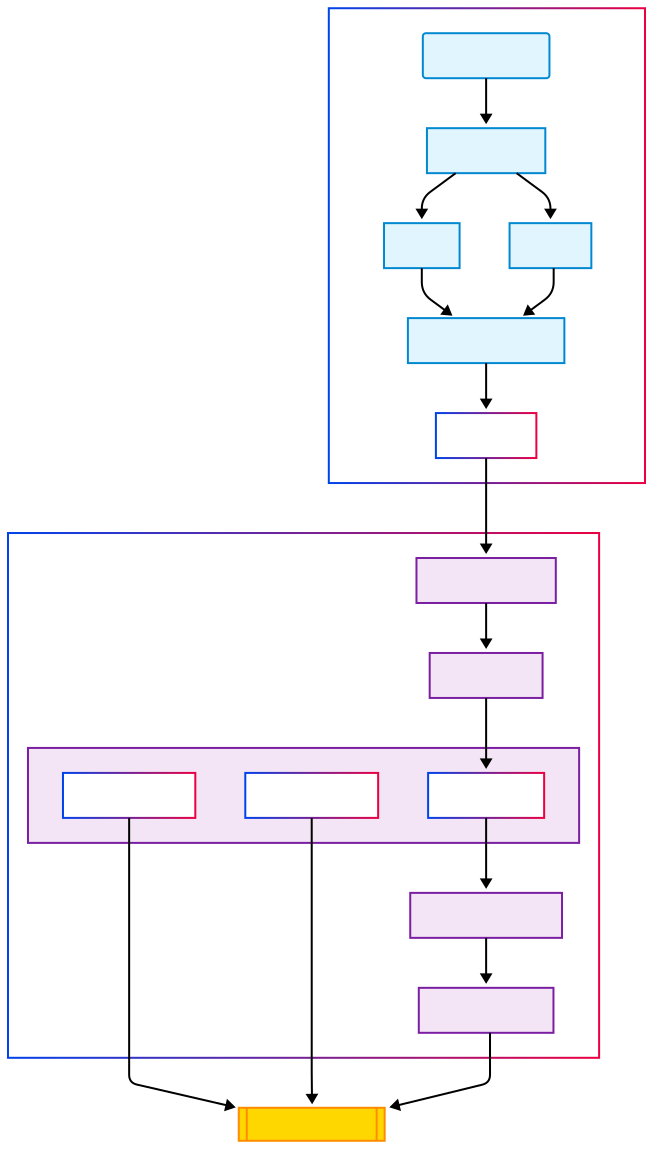
\includegraphics[width=0.85\textwidth]{img/user-diagram-flow}
\caption{High level workflow showing user interaction and data processing}
  \label{fig:user-flow}
\end{figure}

\subsection{Evaluation Framework}\label{subsec:evaluation-framework}
The evaluation framework combines standardized criteria with prompt engineering for consistent results. Four dimensions are used with fixed weights that match the implementation:

\begin{itemize}
  \item \textbf{Problem\mbox{-}Solution Fit} (0.30)
  \item \textbf{Business Model \& Market} (0.30)
  \item \textbf{Team \& Execution} (0.25)
  \item \textbf{Pitch Quality} (0.15)
\end{itemize}

Each dimension evaluates five aspects and yields a numeric score, plus strengths and improvements. Table~\ref{tab:criteria} summarizes the criteria and aspects used.

\begin{table}[H]
  \centering
  \caption{Evaluation criteria and aspects (summary)}
  \label{tab:criteria}
  \begin{tabular}{p{4cm} p{9cm}}
    \toprule
    \textbf{Criterion} & \textbf{Aspects} \\
    \midrule
    Problem\mbox{-}Solution Fit & Problem definition clarity; solution innovation; market understanding; competitive advantage; value proposition \\
    Business Model \& Market & Revenue model; market size \& growth; go-to-market strategy; customer acquisition; scalability potential \\
    Team \& Execution & Team capability; domain expertise; track record; resource management; implementation plan \\
    Pitch Quality & Clarity \& structure; data \& evidence; story \& engagement; Q\&A performance; overall persuasiveness \\
    \bottomrule
  \end{tabular}
\end{table}

The four dimensional processing flow is illustrated in Figure~\ref{fig:eval-flow}. This diagram matches the implemented single provider evaluation pipeline.

\paragraph{Takeaway} Fixed criteria and weights drive all evaluation results and enable reproducible comparisons.

\begin{figure}[H]
  \centering
  \includegraphics[width=0.9\textwidth]{img/eval-flow}
\caption{Evaluation and processing flow across four criteria}
  \label{fig:eval-flow}
\end{figure}

\subsection{AI Integration Strategy}\label{subsec:ai-integration-strategy}
The system uses GPT\,4 through OpenAI's API. Prompts return constrained JSON for reliable parsing. Ensemble or multi-provider evaluation is not part of the current implementation. It is left as future work if needed by the study design.

\paragraph{Prompt calibration} Initial evaluations showed a central tendency around 7/10. To improve spread and validity, we calibrated the scoring prompt. We added rubric anchors for the 1--10 scale. We added evidence gating that caps aspect scores at 4 when specifics are missing. We score aspects first and compute the criterion score as the rounded average. We also use a lower sampling temperature for scoring. The current configuration is tracked as \texttt{PROMPT\_VERSION = criteria\textrm{-}v1.2} and recorded in evaluation metadata.

\paragraph{Error handling} OpenAI calls use retries with exponential backoff for rate limits and transient failures. Responses are validated and mapped into strict application schemas before persistence.

\subsection{Data Models and Storage Architecture}\label{subsec:data-models-and-storage-architecture}
Convex stores pitches and user favorites with schema validation and indexed access. Each document is scoped by user and organization. Q\&A pairs are persisted with each pitch and reused when building evaluation input. Queries update the UI reactively without polling.

\paragraph{Schema overview} The \texttt{pitches} table stores the title, normalized text, type, and status. It also stores structured evaluation results, Q\&A pairs, organization id, user id, author name, and timestamps. Indexes include \texttt{by\_org}, \texttt{by\_user}, \texttt{by\_user\_org}, and \texttt{search\_title}. The \texttt{userFavorites} table links users and pitches with composite indexes.

\subsection{API Endpoints and Server Functions}\label{subsec:api-and-server}
\textbf{Next.js API routes}
\begin{itemize}
  \item \texttt{/api/evaluate} evaluates text using GPT\,4 (Edge runtime)
  \item \texttt{/api/generate-questions} produces up to three follow\mbox{-}up questions
  \item \texttt{/api/evaluate-answers} optional endpoint to update an evaluation using Q\&A responses (not used in the primary UI flow)
  \item \texttt{/api/transcribe} transcribes audio with Whisper\footnote{\url{https://openai.com/research/whisper}}
\end{itemize}

\textbf{Convex functions} (\texttt{convex/pitches.ts})
\begin{itemize}
  \item Mutations: \texttt{create}, \texttt{update}, \texttt{remove}, \texttt{favorite}, \texttt{unfavorite}, \texttt{prefetch}
  \item Queries: \texttt{get}, \texttt{getPitch}, \texttt{getFilteredPitches}, \texttt{getPitchStats}, \texttt{exportCSV}
\end{itemize}

\paragraph{Q\&A generation design} The question generator asks for 1--3 high priority, evidence seeking questions. It returns a structured JSON list tagged to an evaluation dimension. The route uses a lower sampling temperature for stability. If the model returns plain text, a numbered list fallback parser extracts up to three items. This improves evidence capture for the calibrated rubric without changing the original pitch content.

\paragraph{Takeaway} The primary path is transcribe (if audio) \textrightarrow{} generate questions \textrightarrow{} answer \textrightarrow{} evaluate \textrightarrow{} store.

\section{Authentication and Authorization Implementation}
Clerk handles sign in, session management, and organization contexts. Middleware protects routes and injects identity on the server. All Convex reads and writes are scoped by \texttt{userId} and \texttt{orgId}, which provides row level isolation without custom role tables.

\paragraph{Takeaway} Middleware protects app routes and row-level scoping enforces data isolation without complex roles.

\section{User Interface Implementation}
The frontend uses Next.js 15, React 18, and Tailwind CSS\footnote{\url{https://tailwindcss.com}}. Route groups organize the app into dashboard, pitch, and auth areas. Shared UI components live under \texttt{src/components/ui}; feature components live under \texttt{src/components/shared}. Lists support favorites, search, and filtering by score or date. The pitch view renders numeric scores and qualitative feedback with generated follow\mbox{-}up questions.

The pitch creation flow is shown in Figure~\ref{fig:user-flow-pitch}. It covers text input and audio uploads, Q\&A generation, evaluation, and Convex storage. In production use, the Q\&A step is required to capture missing evidence before scoring.

\begin{figure}[H]
  \centering
  \includegraphics[width=0.9\textwidth]{img/user-flow-pitch}
\caption{Pitch creation flow with Q\&A generation and Convex storage}
  \label{fig:user-flow-pitch}
\end{figure}

\paragraph{Takeaway} The UI guides users through a short, consistent flow and surfaces structured scores and feedback.

\section{Performance, Deployment, and Reliability}
\textbf{Performance} Virtualized lists keep lists responsive with large datasets. Code splitting defers non-critical UI. Reactive queries avoid manual polling.

\textbf{Deployment} API routes run on the Edge runtime where configured. Environment variables include the Convex URL, Clerk keys, and OpenAI API key. The same code paths run in development and production for result comparability.

\textbf{Reliability} API routes return clear error messages. The UI surfaces actionable feedback without exposing internal details.

\paragraph{Takeaway} Performance and deployment choices favor responsiveness and consistent behavior across environments.

\section{Implementation Results and User Experience}\label{sec:results}
Text-based evaluations typically complete within 30 to 60 seconds. Audio submissions require extra time for transcription. The interface is reactive, and list updates are visible without manual refresh. These results meet the design goals for responsive, consistent assessments suitable for research and iteration.

\paragraph{Scope} This chapter documents the implemented system. It does not cover earlier experiments with NextAuth and PostgreSQL, industry-specific weight profiles, or ensemble evaluation across multiple model providers. Those topics are left for future work and are referenced in the discussion as potential extensions.
% (Diagram source details moved to appendix for brevity.)

% chapters/4-evaluation.tex
\chapter{Evaluation and Results}
\label{ch:evaluation}

This chapter evaluates the Pista system by comparing it with Winds2Ventures (W2V)\footnote{\url{https://w2v.network/}}, the partner evaluation system introduced in Chapter~\ref{ch:introduction}. The comparison examines differences in scoring patterns and evaluation approaches between the GenAI-powered system and the partner platform.

Evaluating startup pitches involves subjective judgment and domain expertise. To validate the Pista system, comparison with an existing evaluation platform provides insights into how GenAI approaches differ from human-driven assessment methods.

The comparison examined differences in scoring patterns, evaluation consistency, and assessment approaches between the two systems. The analysis focused on understanding where each system shows strengths and limitations.

Comparing GenAI evaluation with existing platforms helps understand the practical utility and limitations of automated assessment tools for startup pitch evaluation.

The comparison addressed three key questions:
\begin{enumerate}
    \item How do Pista scores compare with W2V assessments?
    \item What patterns emerge in the scoring differences?
    \item What are the practical implications for using GenAI evaluation tools?
\end{enumerate}

\section{Methodology and Experimental Design}
\label{sec:methodology}

All results in this chapter use the calibrated scoring prompt (\texttt{PROMPT\_VERSION = criteria\textrm{-}v1.2}) with rubric anchors, evidence gating, aspect first scoring, and a lower sampling temperature for scoring. When Q\&A is enabled, the question generator asks for 1--3 structured, evidence seeking questions and accepts JSON or a numbered list fallback.

\subsection{Metrics}
To evaluate distribution quality and alignment, the analysis reports:
\begin{itemize}
  \item \textbf{Score concentration}: share of exact 7.0 scores before/after calibration
  \item \textbf{Dispersion}: variance or IQR per criterion
  \item \textbf{Rank alignment}: Kendall's $\tau$ with baseline/commercial assessments
  \item \textbf{Evidence sensitivity}: proportion of scores $\leq 4$ when specific evidence is missing
\end{itemize}

\section{Future Work: Ensemble Evaluation}
The current implementation uses a single provider (GPT\,4) with rubric anchored prompts. A practical extension is an ensemble across multiple models to improve stability and evidence coverage:
\begin{itemize}
  \item \textbf{Providers}: Add adapters for OpenAI, Anthropic, and Google; run all providers per criterion in parallel.
  \item \textbf{Aggregation Policy}: Aggregate aspect scores via trimmed mean (e.g., 20\% trim if $\geq$3 providers), then average to the criterion score; record provenance.\footnote{Bump \texttt{POLICY\_VERSION} to \texttt{scoring-policy-v3}.}
  \item \textbf{Disagreement Flags}: If interquartile range across provider scores exceeds a threshold, mark the criterion as low confidence.
  \item \textbf{Adjudication (Optional)}: For flagged criteria, use an adjudicator prompt to merge rationales into the final JSON.
  \item \textbf{Disagreement-Driven Q\&A}: When flagged, generate 1--3 targeted questions for the highest-variance aspects and re-score on answers.
  \item \textbf{Reporting}: Compare ensemble vs. single provider on score dispersion and Kendall's $\tau$ against the baseline (W2V), and document cost/latency trade-offs.
\end{itemize}

\subsection{Dataset Selection and Characteristics}
\label{subsec:dataset}

Twenty-two startup pitches from university entrepreneurship competitions were evaluated by both systems. University competition pitches provided consistent content and format, enabling direct comparison between the two evaluation approaches.

Both systems evaluated all 22 pitches, covering diverse sectors including technology, healthcare, agriculture, and consumer services.

The pitches were obtained through university entrepreneurship programs with appropriate permissions for research use.

Each pitch contained the fundamental components required for comprehensive startup evaluation: clearly defined problem statements, proposed solution descriptions, market opportunity analysis, team capability presentations, and business model articulation. The standardized competition format ensured consistent information availability across all evaluated pitches, facilitating meaningful cross-system comparison.

\subsection{Evaluation Framework Comparison}
\label{subsec:frameworks}

Fundamental differences in evaluation architecture between the two systems necessitated careful methodological consideration for comparative analysis. Each platform employs distinct assessment criteria and weighting mechanisms that reflect different philosophical approaches to startup evaluation.

\subsubsection{Pista Evaluation Framework}

The Pista system employs a four-dimensional weighted assessment structure designed to capture critical aspects of startup viability. The dimensional weighting was calibrated based on venture capital research findings and established industry evaluation practices.

The assessment framework comprises four weighted dimensions:
\begin{enumerate}
    \item \textbf{Problem-Solution Fit (30\% weight)}: Examination of problem definition clarity, solution innovation depth, market understanding sophistication, competitive differentiation strength, and value proposition coherence.

    \item \textbf{Business Model \& Market (30\% weight)}: Analysis of revenue model sustainability, market size estimation credibility, go-to-market strategy feasibility, customer acquisition viability, and scalability potential.

    \item \textbf{Team \& Execution (25\% weight)}: Assessment of team competency profiles, domain expertise relevance, historical performance indicators, resource allocation efficiency, and implementation strategy depth.

    \item \textbf{Pitch Quality (15\% weight)}: Evaluation of presentation structure, evidence integration effectiveness, narrative coherence, and persuasive communication quality.
\end{enumerate}

Quantitative scores are generated on a standardized 1-10 scale for each dimension, accompanied by qualitative feedback containing specific improvement recommendations. The final assessment emerges through weighted aggregation of dimensional scores.

\subsubsection{Winds2Ventures Evaluation Framework}

The platform operates through a nine-criteria assessment methodology focused on investment readiness and commercial viability indicators. Each evaluation criterion contributes to an aggregate "Investibility" rating that reflects overall investment attractiveness from a professional investor perspective.

The evaluation criteria encompass:
\begin{enumerate}
    \item \textbf{Problem Clarity}: Assessment of problem definition precision and market relevance
    \item \textbf{Solution Viability}: Analysis of proposed solution feasibility and effectiveness potential
    \item \textbf{Market Size Estimation}: Evaluation of addressable market opportunity and growth projections
    \item \textbf{Competitive Advantages}: Examination of differentiation strategies and sustainable positioning
    \item \textbf{Team Assessment}: Analysis of team competencies, experience, and execution capabilities
    \item \textbf{Business Model Viability}: Investigation of revenue mechanisms and sustainability factors
    \item \textbf{Go-To-Market Strategy}: Review of market entry approaches and scaling methodologies
    \item \textbf{Competitive Landscape}: Assessment of market dynamics and competitive positioning
    \item \textbf{Funding Ask and Use}: Analysis of capital requirements and allocation strategies
\end{enumerate}

The W2V evaluation process involves experienced investors and business professionals who contribute extensive industry knowledge and practical investment experience. This human expertise emphasizes realistic market dynamics and execution risk factors, typically resulting in more conservative assessment patterns than algorithmic evaluation approaches.

\subsection{Score Mapping and Comparison Methodology}
\label{subsec:methodology-approach}

The divergent evaluation frameworks presented methodological challenges for direct comparative analysis. To address these complexities, a conservative analytical approach was adopted that focused primarily on overall assessment scores rather than attempting complex dimensional mappings between disparate criteria sets.

The comparison methodology centered on Pista's weighted overall scores against W2V's Investibility ratings. Both systems generate standardized 1-10 scale assessments, facilitating direct numerical comparison without requiring complex score transformations or normalization procedures. This approach preserved the integrity of each system's underlying evaluation philosophy while enabling meaningful quantitative analysis.

\section{Results and Analysis}
\label{sec:results}

\subsection{Overall Performance Patterns}
\label{subsec:performance}

The comparative analysis revealed systematic differences between evaluation systems that extend beyond random variation, suggesting fundamental divergences in assessment philosophy and methodology. These patterns emerged consistently across all evaluated pitches, indicating structural rather than circumstantial differences.

Across all 22 evaluated pitches, Pista consistently generated higher scores than W2V, with no exceptions observed. The average scoring differential measured +1.70 points, representing a substantial and systematic bias that suggests underlying philosophical differences in evaluation approach rather than random measurement variation.

\begin{table}[ht]
    \centering
    \caption{Comprehensive Score Comparison Analysis}
    \label{tab:score-comparison}
    \begin{tabular}{lccc}
        \toprule
        \textbf{System} & \textbf{Average Score} & \textbf{Score Range} & \textbf{Standard Deviation} \\
        \midrule
        Pista & 6.81/10 & 6.0-8.0 & 0.50 \\
        Winds2Ventures & 5.11/10 & 4.3-6.4 & 0.63 \\
        \midrule
        \textbf{Difference} & +1.70 & - & - \\
        \bottomrule
    \end{tabular}
\end{table}

Analysis of scoring distributions revealed significant differences in discrimination capabilities between the evaluation systems.

Pista scores demonstrated clustering within a relatively narrow 6.0-8.0 range, producing a standard deviation of 0.50. In contrast, W2V scores exhibited broader distribution spanning 4.3-6.4 points with higher variance ( = 0.63). These distribution patterns suggest different approaches to quality discrimination, with W2V demonstrating greater sensitivity to quality variations across evaluated pitches.

\subsection{Systematic Bias Identification}
\label{subsec:bias}

Detailed pattern analysis exposed several consistent systematic biases that significantly influence GenAI evaluation reliability and practical deployment viability.

\subsubsection{Systematic Optimism Bias}

The most prominent pattern is optimism in GenAI scoring. As noted above, Pista scored higher in all 22 cases (+1.70 average difference). This directional bias spans pitch quality and industry sectors, which suggests systematic rather than circumstantial influences.

Several factors likely contribute to this optimism bias. Training data composition may overrepresent successful startup examples, creating algorithmic tendencies toward positive assessment. Additionally, GenAI systems may lack the sophisticated risk evaluation capabilities that characterize experienced human evaluators, who integrate market realities and execution challenges developed through practical investment experience.

\subsubsection{Limited Discriminative Power}

A striking pattern emerged in score distribution analysis: 66.7\% of Pista evaluations (15/22 pitches) received identical overall scores of exactly 7.0/10. This substantial clustering indicates critical algorithmic limitations in quality differentiation capabilities. Rather than reflecting genuine quality similarities among evaluated pitches, this pattern suggests algorithmic convergence toward a default "safe" assessment value.

Such limited discrimination presents significant challenges for practical investment applications. Professional investors require granular quality distinctions to effectively prioritize opportunities and allocate limited evaluation resources. When most assessments converge on identical scores, the system fails to provide the nuanced discrimination essential for informed decision-making.

\begin{table}[ht]
    \centering
    \caption{Systematic Bias Analysis}
    \label{tab:bias-analysis}
    \begin{tabular}{lccc}
        \toprule
        \textbf{Bias Category} & \textbf{Frequency} & \textbf{Impact Magnitude} & \textbf{Strategic Implications} \\
        \midrule
        GenAI Evaluation Optimism & 22/22 (100\%) & +1.70 points average & Systematic over-confidence \\
        Limited GenAI Discrimination & 15/22 (66.7\%) & Identical scores & Insufficient quality differentiation \\
        Commercial Conservatism & 22/22 (100\%) & Consistent lower scoring & Risk-aware assessment \\
        \bottomrule
    \end{tabular}
\end{table}

\subsection{Dimensional Performance Analysis}
\label{subsec:dimensional}

\begin{table}[ht]
    \centering
    \caption{Pista Dimensional Performance Analysis}
    \label{tab:dimensional-analysis}
    \begin{tabular}{lcc}
        \toprule
        \textbf{Dimension} & \textbf{Pista Average} & \textbf{Performance Characteristics} \\
        \midrule
        Problem-Solution Fit & 7.1/10 & Highest dimensional performance \\
        Business Model \& Market & 6.9/10 & Consistently strong assessment \\
        Pitch Quality & 6.8/10 & Stable evaluation patterns \\
        Team \& Execution & 6.6/10 & Comparatively lower performance \\
        \bottomrule
    \end{tabular}
\end{table}

Dimensional analysis exposed systematic performance variations across evaluation categories, revealing specific algorithmic strengths and limitations. Problem-Solution Fit achieved the highest average scores (7.1/10), suggesting that GenAI systems demonstrate particular effectiveness in analyzing business logic structures and solution viability assessments.

Conversely, Team \& Execution consistently received the lowest dimensional scores (6.6/10), indicating algorithmic challenges in assessing human capital factors. This performance gap likely reflects GenAI limitations in evaluating intangible elements such as leadership depth, team dynamics, and execution track records. These are factors that human evaluators often assess through experience based pattern recognition and interpersonal judgment.

\section{Case Study Analysis}

\begin{table}[ht]
    \centering
    \caption{Comparative Case Study Analysis}
    \label{tab:case-studies}
    \begin{tabular}{lp{3cm}cccp{4cm}}
        \toprule
        \textbf{Company} & \textbf{Description} & \textbf{Pista Score} & \textbf{W2V Score} & \textbf{Difference} & \textbf{Primary Evaluation Focus Difference} \\
        \midrule
        Coontent & Marketing automation B2B SaaS platform & 6.5/10 & 5.3/10 & +1.2 & GenAI: Innovation potential vs W2V: Market competition \\
        \midrule
        Serenity & GenAI-powered mental wellness platform & 6.9/10 & 6.1/10 & +0.8 & GenAI: Market opportunity vs W2V: Regulatory challenges \\
        \midrule
        CampoRapido & Agricultural technology platform & 7.0/10 & 4.5/10 & +2.5 & GenAI: Problem-solution fit vs W2V: Market readiness \\
        \midrule
        Corptech & Industrial technology platform & 8.0/10 & 6.0/10 & +2.0 & GenAI: Technical innovation vs W2V: Execution readiness \\
        \bottomrule
    \end{tabular}
\end{table}

Case study analysis across diverse industry sectors revealed three distinct patterns that illuminate fundamental evaluation differences. First, scoring differentials ranged from 0.8 to 2.5 points, with regulated industries (Serenity: +0.8) showing smaller gaps and agricultural technology (CampoRapido: +2.5) exhibiting the largest disparities. Second, evaluation focus differed systematically: Pista emphasized innovation potential and technical merit, while W2V prioritized practical deployment challenges including regulatory compliance, market readiness, and execution risks. Third, even high-performing pitches like Corptech, which received the highest scores from both systems (8.0 Pista, 6.0 W2V), maintained substantial scoring gaps (+2.0), confirming that evaluation differences stem from systematic philosophical divergences rather than pitch quality variations.

\section{Discussion and Deployment Implications}

The comparison revealed consistent differences between Pista and W2V scoring approaches. As shown above, Pista scores were higher on average, which suggests a tendency toward optimistic assessment. The following sections discuss practical implications and use cases.

\subsection{Systematic Bias Analysis}
\label{sec:bias-analysis}

The comparison reveals three main patterns in how Pista differs from W2V in its evaluation approach.

\subsubsection{Universal GenAI Optimism}
\label{subsec:optimism}

Pista's consistent higher scoring (22/22 pitches) was interpreted as suggesting a training bias toward positive examples; it was also considered to indicate insufficient risk assessment capabilities. This optimism was identified as limiting utility for investment decision contexts.

The universal directional bias indicates that GenAI systems may be fundamentally designed to highlight opportunities rather than assess risks. This could result from training data that emphasizes successful startup characteristics without adequate representation of failure patterns. Commercial evaluators, by contrast, integrate market realities and execution challenges that create more conservative assessments.

\subsubsection{Score Convergence Limitations}
\label{subsec:convergence}

The concentration of 66.7\% of scores at exactly 7.0/10 was identified as indicating critical algorithmic limitations in quality differentiation. This clustering was interpreted as suggesting the evaluation model defaults to a "safe" middle-high score regardless of actual pitch quality variations.

This convergence pattern creates several practical challenges. Investment decisions require discrimination between opportunities to allocate resources effectively. When most evaluations receive identical scores, the system fails to provide the granular assessment needed for professional deployment. The algorithmic tendency toward convergence may reflect conservative design choices that prioritize consistency over discrimination.

\subsubsection{Risk Assessment Variations}
\label{subsec:risk}

Maximum disagreements occurred in technology and service platforms where commercial evaluators emphasized execution risks and market competition factors that GenAI evaluation appears to underweight.

GenAI systems focus on innovation potential and technical merit while underweighting execution challenges and competitive dynamics. Commercial platforms incorporate broader risk factors developed through investment experience. This difference reflects fundamental evaluation philosophy variations rather than calibration issues.

\subsection{Deployment Strategy Implications}
\label{sec:deployment}

The systematic differences suggest complementary rather than competing deployment strategies. Given GenAI's operational advantages (speed, cost, accessibility) and limitations (optimism bias, poor discrimination), strategic deployment becomes crucial.

\subsubsection{Appropriate GenAI Applications}
\label{subsec:ai-applications}

GenAI evaluation systems demonstrate clear advantages for specific use cases that align with their operational strengths and philosophical characteristics:

\textbf{Early-stage entrepreneur feedback and pitch development support}: The systematic optimism bias becomes advantageous for encouraging entrepreneurs and providing constructive feedback without discouraging innovation attempts.

\textbf{High-volume initial screening where broad categorization suffices}: The speed and cost advantages enable processing large numbers of pitches where precise discrimination is less critical than general quality assessment.

\textbf{Educational contexts where encouraging feedback promotes learning}: The consistent scoring patterns provide stable feedback that supports learning environments without creating discouraging assessment variations.

\subsubsection{Commercial Evaluation Requirements}
\label{subsec:commercial-requirements}

Commercial evaluation platforms demonstrate capabilities that remain essential for professional investment contexts:

\textbf{Investment decision-making requiring realistic risk assessment}: The broader score distribution and conservative assessment approach align with professional investment requirements for risk evaluation.

\textbf{Applications demanding granular quality discrimination}: The varied scoring patterns enable the discrimination needed for resource allocation and opportunity prioritization in competitive markets.

\textbf{Complex market sectors}: Technology and B2B services may benefit from the domain expertise that platforms like W2V provide through experienced evaluators.

\subsubsection{Hybrid Strategy Optimization}
\label{subsec:hybrid}

Using GenAI tools like Pista for initial feedback and platforms like W2V for more detailed assessment could combine the speed of GenAI with the nuanced evaluation of experienced assessors.

The hybrid strategy addresses both system limitations and advantages. GenAI systems handle high-volume screening efficiently while commercial systems provide the discrimination and risk assessment needed for investment decisions. This complementary approach maximizes overall evaluation system effectiveness.

\subsection{Evaluation Quality vs. Operational Efficiency Trade-offs}
\label{sec:tradeoffs}

The evaluation reveals a fundamental trade-off between operational efficiency and assessment quality. GenAI evaluation provides substantial operational advantages but at the cost of evaluation precision and realistic risk assessment.

\subsubsection{Operational Advantages}
\label{subsec:advantages}

GenAI's speed (30-60 seconds), cost (\$0.10-0.15), and availability (24/7) enable applications impossible with traditional evaluation methods, democratizing access to startup feedback. These advantages create entirely new use cases that were previously economically unfeasible.

The operational efficiency enables applications such as real-time pitch feedback during development, continuous iteration support, and accessible evaluation for entrepreneurs who cannot afford professional assessment services. This democratization effect represents a significant value creation opportunity.

\subsubsection{Quality Limitations}
\label{subsec:limitations}

Score convergence and optimism bias severely limit GenAI utility for contexts requiring discriminative assessment or realistic risk evaluation. These limitations constrain professional deployment opportunities where quality assessment is critical.

The quality limitations become particularly problematic when AI evaluation results influence significant decisions. Investment contexts require accurate risk assessment and quality discrimination that current GenAI systems cannot provide reliably. This constrains professional deployment until these limitations are addressed.

\subsubsection{Strategic Trade-off Management}
\label{subsec:strategy}

These differences suggest GenAI evaluation and traditional platforms serve different purposes, with each being more suitable for specific use cases rather than directly competing.

Successful deployment requires matching GenAI capabilities with appropriate use cases while using commercial evaluation where quality requirements exceed GenAI capabilities. This strategic approach enables value creation through GenAI advantages while maintaining quality standards where needed.

\section{Threats to Validity}
\label{sec:threats}

This section reflects on limitations that may affect interpretation of results.

\subsection{Internal Validity}
The evaluation uses identical pitch content across systems, but prompts and calibration choices may influence outcomes. We reduced this risk with rubric anchors, evidence gating, and a fixed temperature, yet residual effects may remain. Future work can ablate each calibration component to measure its impact.

\subsection{Construct Validity}
The four-dimension rubric approximates startup quality but cannot capture all factors. Some human judgments, such as leadership depth and execution history, are hard to encode. We mitigated this by adding a required Q\&A step to collect missing evidence before scoring.

\subsection{External Validity}
The dataset contains 22 university competition pitches. Results may not generalize to all sectors or later-stage ventures. Expanding the dataset and including investor-written memos would improve generalizability.

\subsection{Conclusion Validity}
We report descriptive statistics and qualitative patterns. Larger samples and rank-correlation tests would strengthen claims about dispersion and agreement. We recommend Kendall's $\tau$ for future studies.

\section{Summary}
\label{sec:summary}

This comparative evaluation examined systematic differences between GenAI and commercial startup assessment methodologies through analysis of 22 university entrepreneurship competition pitches. The investigation revealed fundamental divergences in evaluation philosophy and practical capabilities between automated and human expert assessment approaches.

\textbf{Principal Findings}:
\begin{itemize}
    \item Universal optimism bias: Pista scored higher than W2V in all cases without exception (22/22 pitches)
    \item Substantial scoring differential: +1.70 average point difference (Pista: 6.81/10, W2V: 5.11/10)
    \item Algorithmic convergence limitation: 66.7\% of GenAI evaluations clustered at identical 7.0/10 scores
    \item Commercial platform demonstrated broader discrimination: 4.3-6.4 scoring range with higher variance
    \item Systematic GenAI tendency toward middle-high score convergence independent of actual quality variations
\end{itemize}

The findings suggest that GenAI evaluation systems like Pista and platforms like W2V have different strengths, making them suitable for different purposes in startup assessment.

% \chapter{Conclusion and Future Work}
\label{ch:conclusion}

This thesis developed Pista, a GenAI-powered startup pitch evaluation system, and compared its performance with Winds2Ventures (W2V). Through evaluation of 22 startup pitches, differences in scoring patterns and evaluation approaches were analyzed.

\section{Key Findings}
\label{sec:key-findings}

\textbf{Systematic GenAI Optimism}: Pista scored higher than Winds2Ventures in 100\% of cases (22/22 pitches), averaging +1.70 points difference. This universal bias indicates fundamental evaluation philosophy differences.

\textbf{Limited Discrimination}: 66.7\% of GenAI evaluations (15/22 pitches) received identical 7.0/10 scores, indicating critical limitations in quality differentiation. Commercial platforms demonstrated broader score distribution (4.3-6.4 range) with superior discrimination capabilities.

\textbf{Dimensional Variations}: GenAI systems performed strongest in Problem-Solution Fit evaluation (7.1/10) but weakest in Team \& Execution assessment (6.6/10), reflecting limitations in evaluating human factors and leadership capabilities.

\section{Deployment Implications}
\label{sec:applications}

The comparison revealed different strengths for each approach. Pista offers fast, consistent evaluation suitable for educational contexts and initial screening. W2V provides more varied scoring that better reflects real-world investment assessment needs.

\section{Research Contributions}
\label{sec:contributions}

This work developed a functional GenAI evaluation system and compared it with an existing evaluation platform. The comparison revealed systematic differences in scoring patterns and highlighted areas where GenAI evaluation shows promise and limitations.

\section{Limitations and Future Work}
\label{sec:limitations}

\textbf{Study Limitations}: The limited sample size (22 pitches) and university competition context may not fully represent professional investment scenarios. Single commercial platform comparison constrains broader generalizability.

\textbf{Future Research}: Larger professional samples, multi-platform analysis, and longitudinal tracking of startup outcomes would strengthen validation. Multimodal capabilities integrating video and audio analysis could address current text-only limitations. Interactive evaluation systems with GenAI-generated follow-up questions would bridge the gap between static analysis and dynamic human assessment.

\section{Conclusion}
\label{sec:conclusion}

The comparison shows that GenAI evaluation systems like Pista can provide useful feedback for entrepreneurs and educational settings, while platforms like W2V offer more nuanced assessment for investment contexts. Each approach has distinct strengths that make them suitable for different use cases.

Future work could focus on improving GenAI evaluation discrimination and reducing scoring convergence while maintaining the speed and accessibility advantages that make such systems valuable for entrepreneurship education and initial pitch development.




\appendix

% \input{help} 

\bibliographystyle{unsrt}                                 
\bibliography{bibliography}

\end{document}